\documentclass[11pt,titlepage]{article}
\usepackage[utf8]{inputenc}
\usepackage[dutch]{babel}
\usepackage{amsmath}
\usepackage{amsfonts}
\usepackage{amssymb}
\usepackage{graphicx}
\usepackage[table,xcdraw]{xcolor}
\usepackage[toc,page]{appendix}
\usepackage{hyperref}
\usepackage{listings}
\usepackage{float}
\usepackage{tikz}
\usetikzlibrary{trees}
\usepackage{tikz-qtree}
\usepackage{graphicx}
\usepackage{fancyref}
\usepackage{wrapfig}
\usepackage{url}
\usepackage{pdflscape}
\usepackage{fancyvrb}
\graphicspath{ {Afbeeldingen/} }
\usepackage{subfig}
\usepackage{tabularx}

\newcolumntype{L}[1]{>{\raggedright\arraybackslash}p{#1}}

%% Sets page size and margins 
\usepackage[a4paper,top=3cm,bottom=3cm,left=3cm,right=3cm,marginparwidth=1.75cm]{geometry}

\author{René van Eendenburg 561378 \cr Derk Wiegerinck 567665}

\title{Demo Documentatie}
\usepackage{titling}

\newcommand{\subtitle}[3]{%
	\posttitle{%
		\par\end{center}
	\begin{center}\large#1\end{center}
	\begin{center}\large#2\end{center}
	\begin{center}\large#3\end{center}
	\vskip0.5em}%
}

\subtitle{HAN Arnhem}{Versie 1}{WOR-World}

\frenchspacing
\sloppy
\begin{document}
\maketitle



\tableofcontents
\clearpage


\section{Inleiding}
Dit document beschrijft wat er nodig is om een simulatie te kunnen bouwen, het starten van de simulatie en het uitvoeren van een demo.

\section{Benodigdheden}
Uw Linux distributie zal Robot Operating System (Ros) moeten ondersteunen. Kijk onder deze \href{https://www.ros.org/reps/rep-0003.html}{link} of uw distributie wordt ondersteund.

Verder zijn de volgende onderdelen benodigd om de simulatie te bouwen en uit te voeren
\begin{itemize}
    \item \href{http://wiki.ros.org/melodic/Installation}{Ros Melodic}
    \item GCC 7.4.0 of hoger
\end{itemize}

\section{Bouwen van de broncode}
Allereerst zult u een workspace moeten hebben. Dit kunt u doen door de volgende commando' s uit te voeren

\begin{verbatim}
$ mkdir -p ~/catkin_ws/src
$ cd ~/catkin_ws/
$ catkin_make
$ source /opt/ros/<distro>/setup.bash
\end{verbatim}

Daarna kunt u de packages in de zojuist aangemaakte src map kopieren. 

\begin{verbatim}
$ cp /directory/to/RobotSimulation/src/* ~/catkin_ws/src
$ catkin_make
$ source devel/setup.bash
\end{verbatim}

\section{Uitvoeren simulatie}
Na het bouwen van de broncode, kan de simulatie worden gestart. Hiervoor opent u een terminal in de workspace en voert u de volgende stappen uit.

\begin{verbatim}
$ cd ~/catkin_ws
$ source devel/setup.bash
$ roslaunch al5d_simulation al5d_simulation.launch 
\end{verbatim}

In deze demo is te zien hoe de beker wordt opgepakt. Daarna wordt de beker naar een nieuwe locatie gebracht en neergezet. Daarna zal de beker weer opgepakt worden en de robot de beker weer meenemen. Om te laten zien dat zwaartekracht ook werkt, wordt de beker losgelaten. Dit zorgt er wel voor dat de demo maar eenmaling kan worden uitgevoerd. Mocht deze nog een keer afgespeeld worden, moet de roslaunch en het demo script opnieuw worden gestart.
\newline
Daarnaast is het mogelijk om de bekerpositie aan te passen in de launch file. Zie hiervoor de Cup1Pos argument.

\section{Behaalde Eisen}
\begin{table}[H]
\centering
\begin{tabular}[H]{|l|l|}
\hline
\rowcolor[HTML]{C0C0C0}
Criteria        &   Aangetoond door:                                                        \\ \hline
PA01-04         &   Alle code is opgebouwd volgens de ROS structuur en style guide.         \\ 
                &   Verder zijn alle onderdelen OO opgebouwd                                \\ \hline
VS01-03         &   SSC32U berichten worden gestuurd naar het request topic en afgehandeld. \\   
                &   Dit is zichtbaar in Rviz dankzij de bewegende robot arm.                \\ \hline
VS04            &   De vertraging commando's per servo of globaal met tijd worden gebruikt  \\ 
                &   in de Demo en worden realistisch afgehandeld.                           \\ \hline
VC01            &   De beker kan op een willekeurige positie worden gezet in de launchfile  \\ \hline
VC03            &   Beker is zichtbaar gemaakt d.m.v. een marker                            \\ \hline
VC04-05         &   De relevante punten van de gripper worden aangeduid met een rode marker \\ \hline
VC06-07         &   De beker marker veranderd van kleur wanneer opgepakt.                   \\ \hline
VC08            &   Zie demo                                                                \\ \hline
VC09-12         &   Alle relevante beker informatie is uit te lezen met rqt\_plot.           \\ 
                &   Lees met rqt\_plot het cup1 topic uit of zie figuur 1                    \\ \hline
VC13            &   Zie demo                                                                \\ \hline
DI01            &   Alle relevante onderdelen worden opgestart met de launchfile            \\ \hline
DI02            &   De bekerpositie is configurabel in de launchfile                        \\ \hline
DI04            &   Demoscript stuurt verschillende commando's met delays naar de demo      \\ \hline

\end{tabular}
\caption{Eisen}
\end{table}

\begin{figure}[H]
\centering
    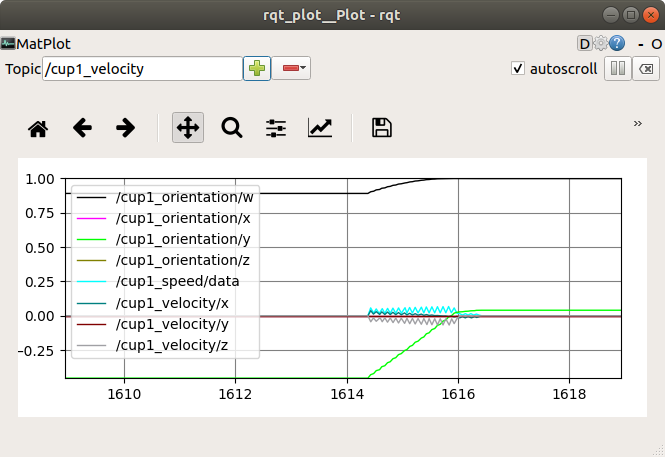
\includegraphics[scale = .4]{rqt_plot.png}
    \caption{rqt\_plot van een gesimuleerde beker}
    \label{figure:al5d_simulation}
\end{figure}

\end{document}
